\chapter{نمودارهای کلاس طراحی}
در این فصل نمودارهای کلاس طراحی همراه با جزییات آن‌ها آورده شده است. به علت جلوگیری از ناخوانا شدن، از مکانیزم بسته‌بندی
\LTRfootnote{Packaging}
استفاده شده است. در هر بسته چند کلاس مرتبط به همراه ارتباطهایشان با کلاس‌های بیرونی قابل مشاهده است.
\section{بسته پروژه}
\begin{figure}[H]
	\centering
	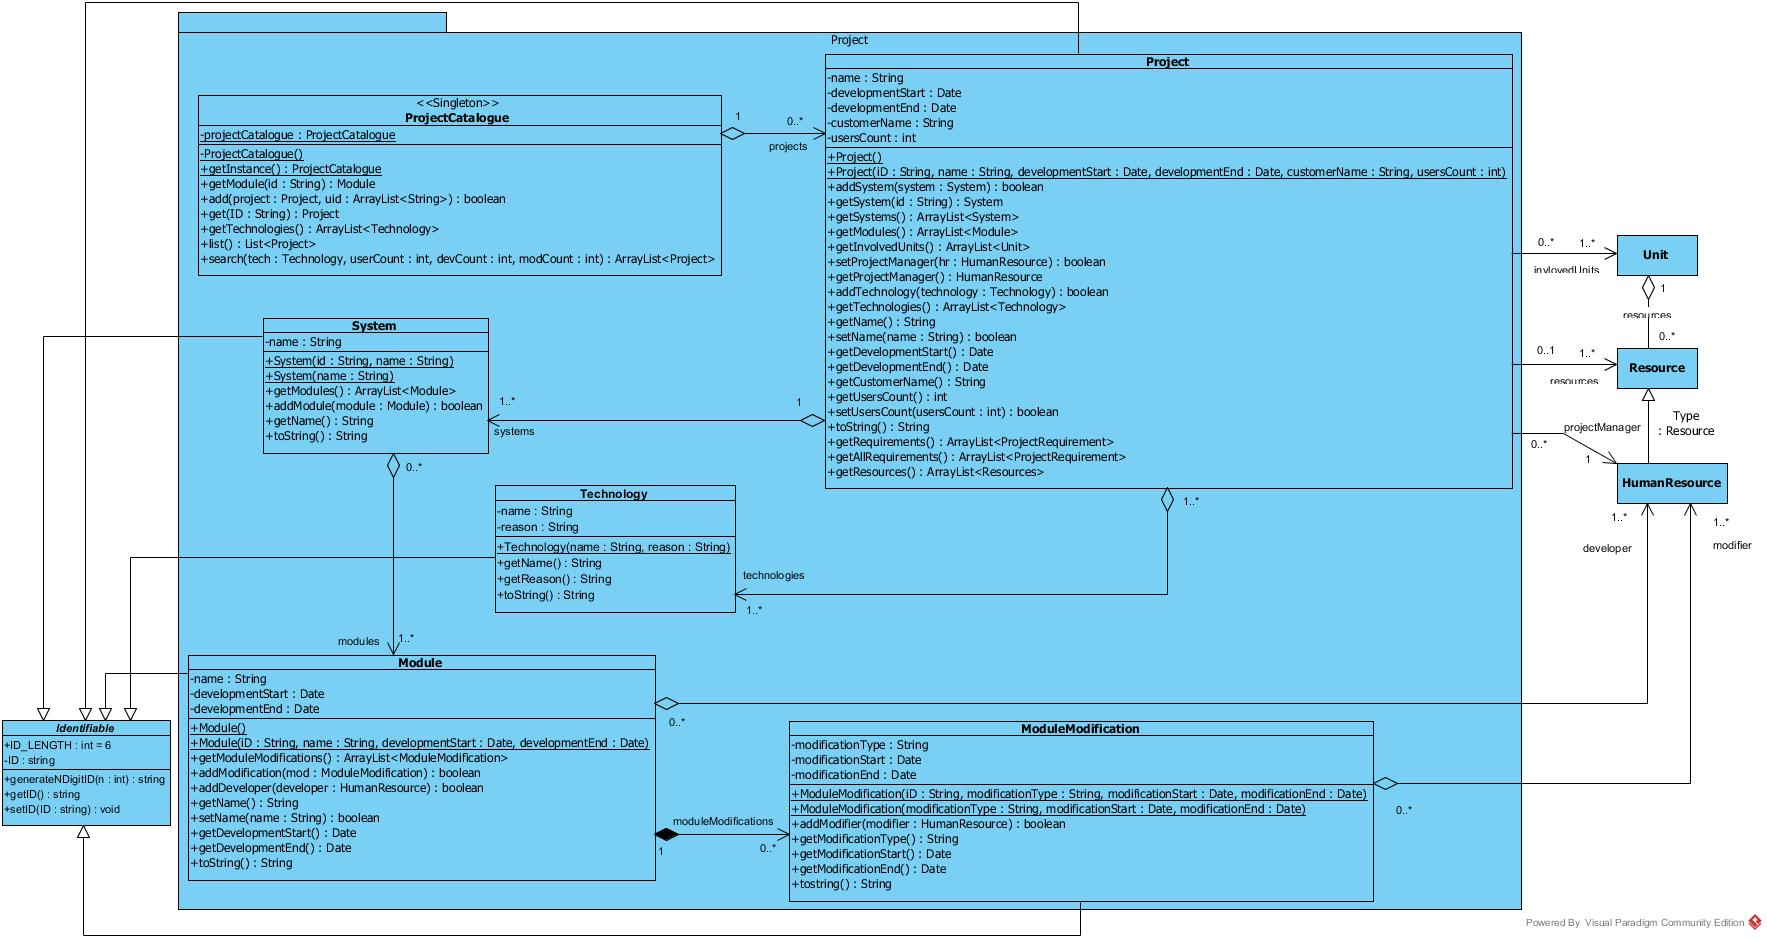
\includegraphics[scale=0.45]{img/class-design/ProjectPackage}
	\caption{صفحه ورود}
\end{figure}

\section{بسته منبع}
\begin{figure}[H]
	\centering
	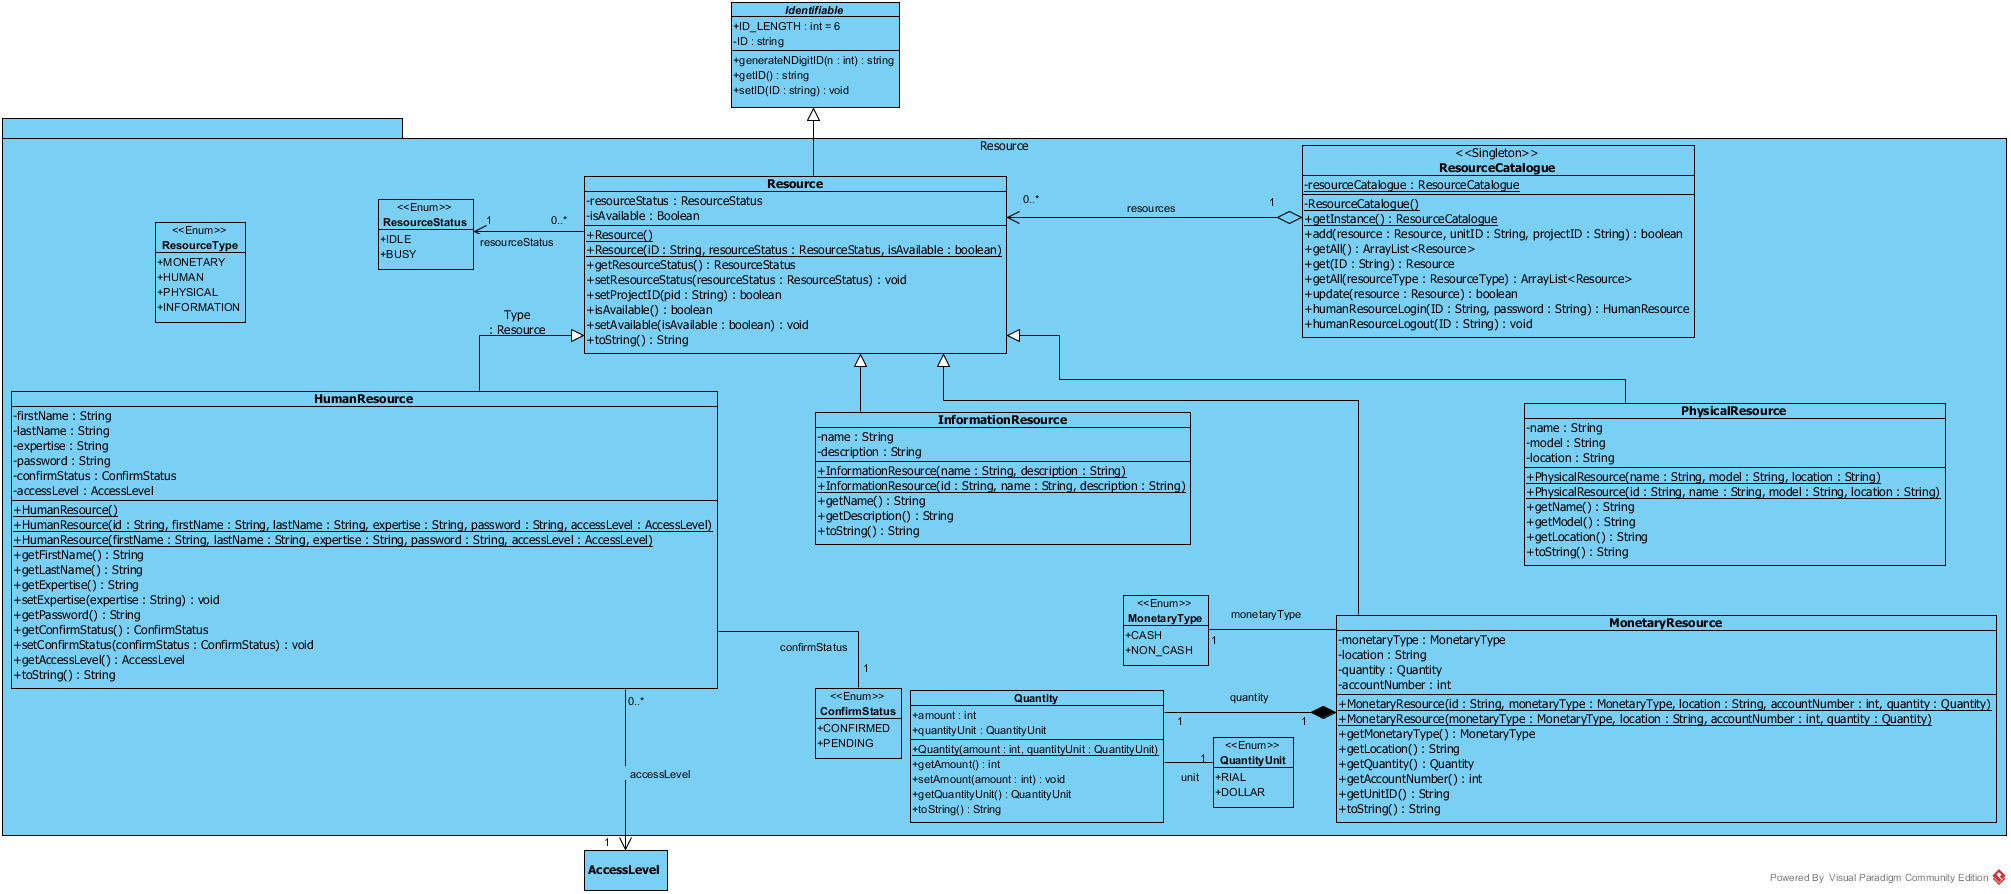
\includegraphics[scale=0.45]{img/class-design/ResourcePackage}
	\caption{بسته منیع}
\end{figure}

\section{بسته واحد}
\begin{figure}[H]
	\centering
	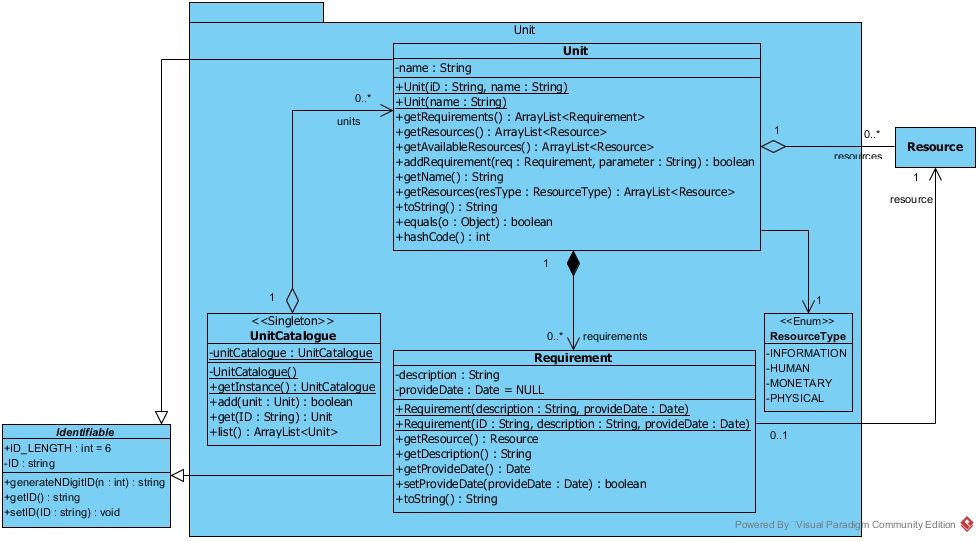
\includegraphics[scale=0.6]{img/class-design/UnitPackage}
	\caption{بسته واحد}
\end{figure}

\section{بسته گزارش}
\begin{figure}[H]
	\centering
	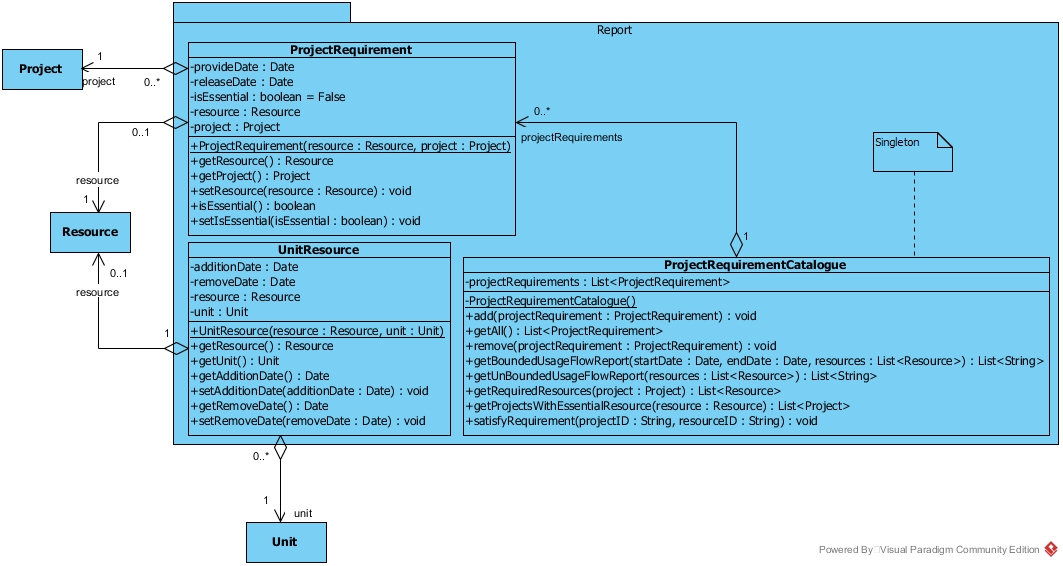
\includegraphics[scale=0.45]{img/class-design/ReportPackage}
	\caption{بسته گزارش}
\end{figure}

\section{بسته دسترسی}
\begin{figure}[H]
	\centering
	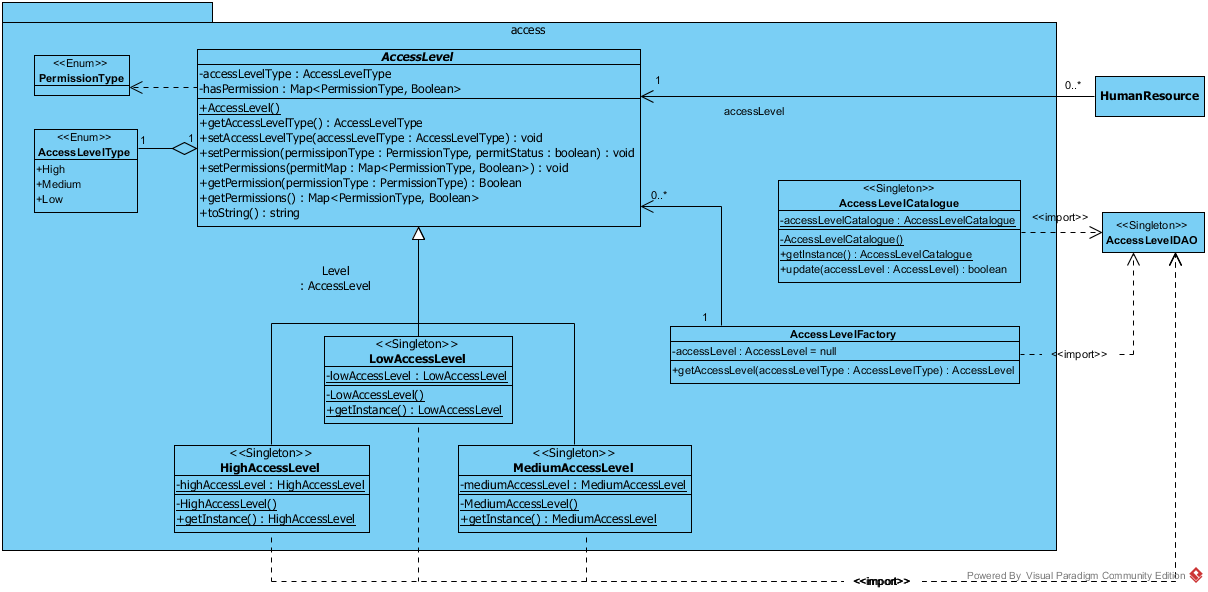
\includegraphics[scale=0.6]{img/class-design/AccessPackage}
	\caption{بسته دسترسی}
\end{figure}

\begin{landscape}
\section{بسته پایگاه‌داده}
از آن‌جایی که کلاس قالب
\LTRfootnote{Template}
 DAO یک واسط است، لازم است که توابع آن در همه‌ی کلاس‌هایی که به آن bind می‌شوند پیاده‌سازی شود. اما با توجه به ملاحظات مربوط به خوانایی و قرارگیری در مستند، از تکرار آن‌ها در کلاس‌های با پسوند DAO خودداری شده است.
\begin{figure}[H]
	\centering
	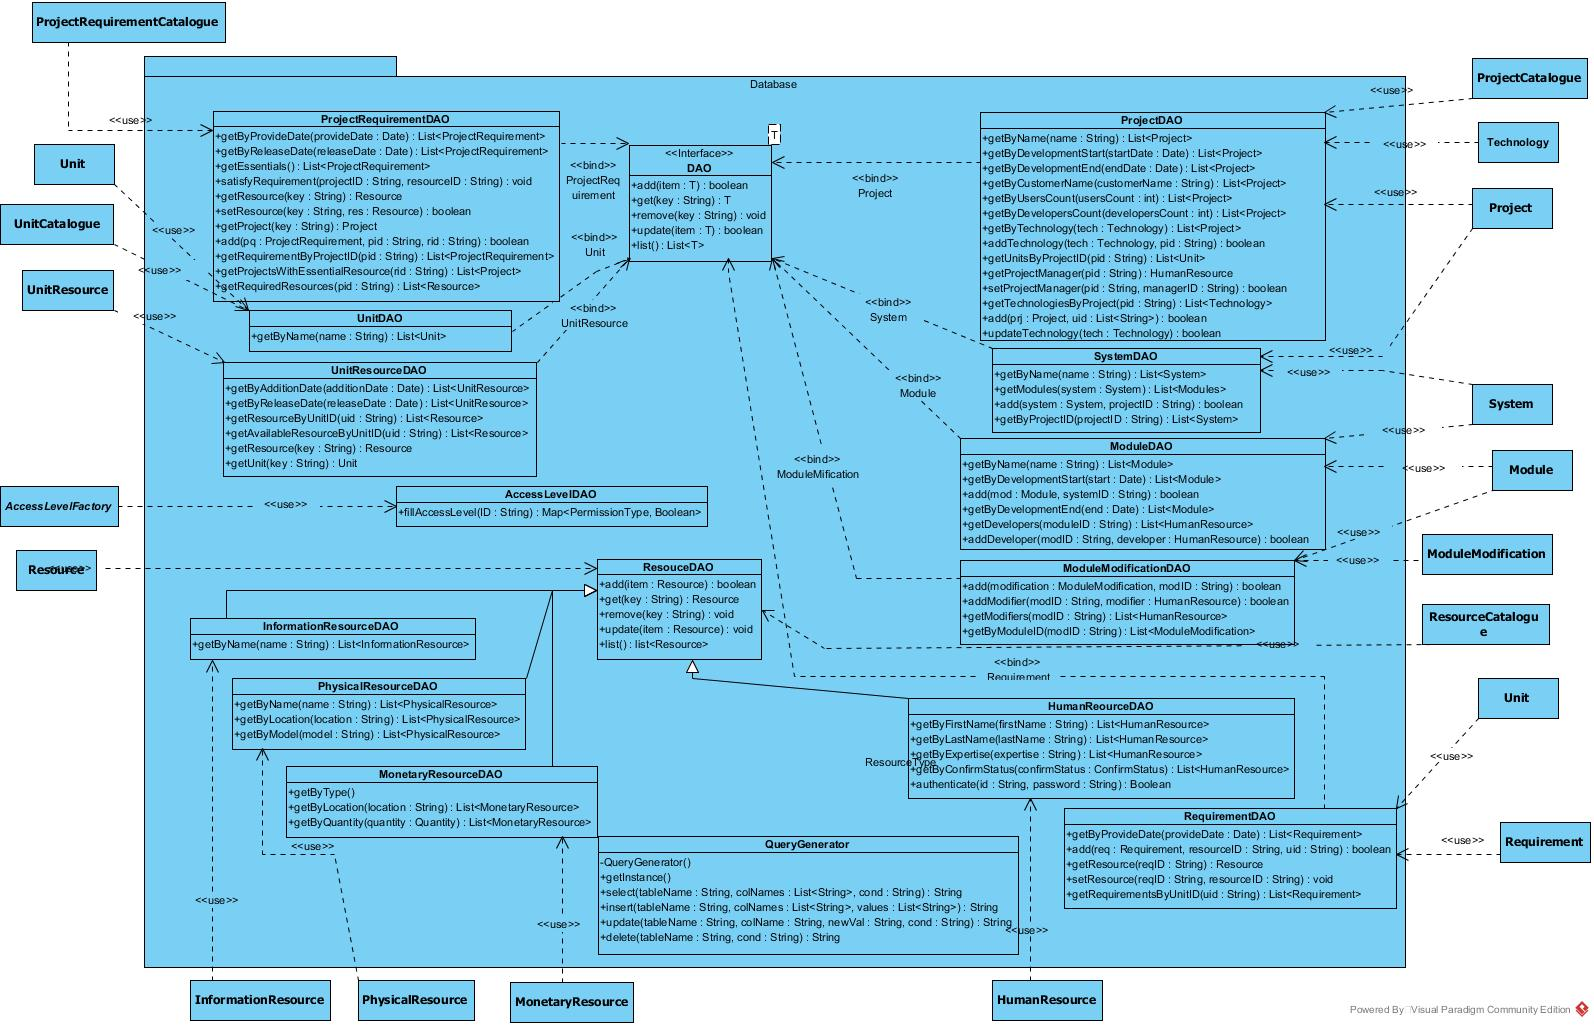
\includegraphics[scale=0.45]{img/class-design/DatabasePackage}
	\caption{بسته پایگاه‌داده}
\end{figure}
\end{landscape}
\section{بسته واسط کاربری}
\begin{figure}[H]
	\centering
%	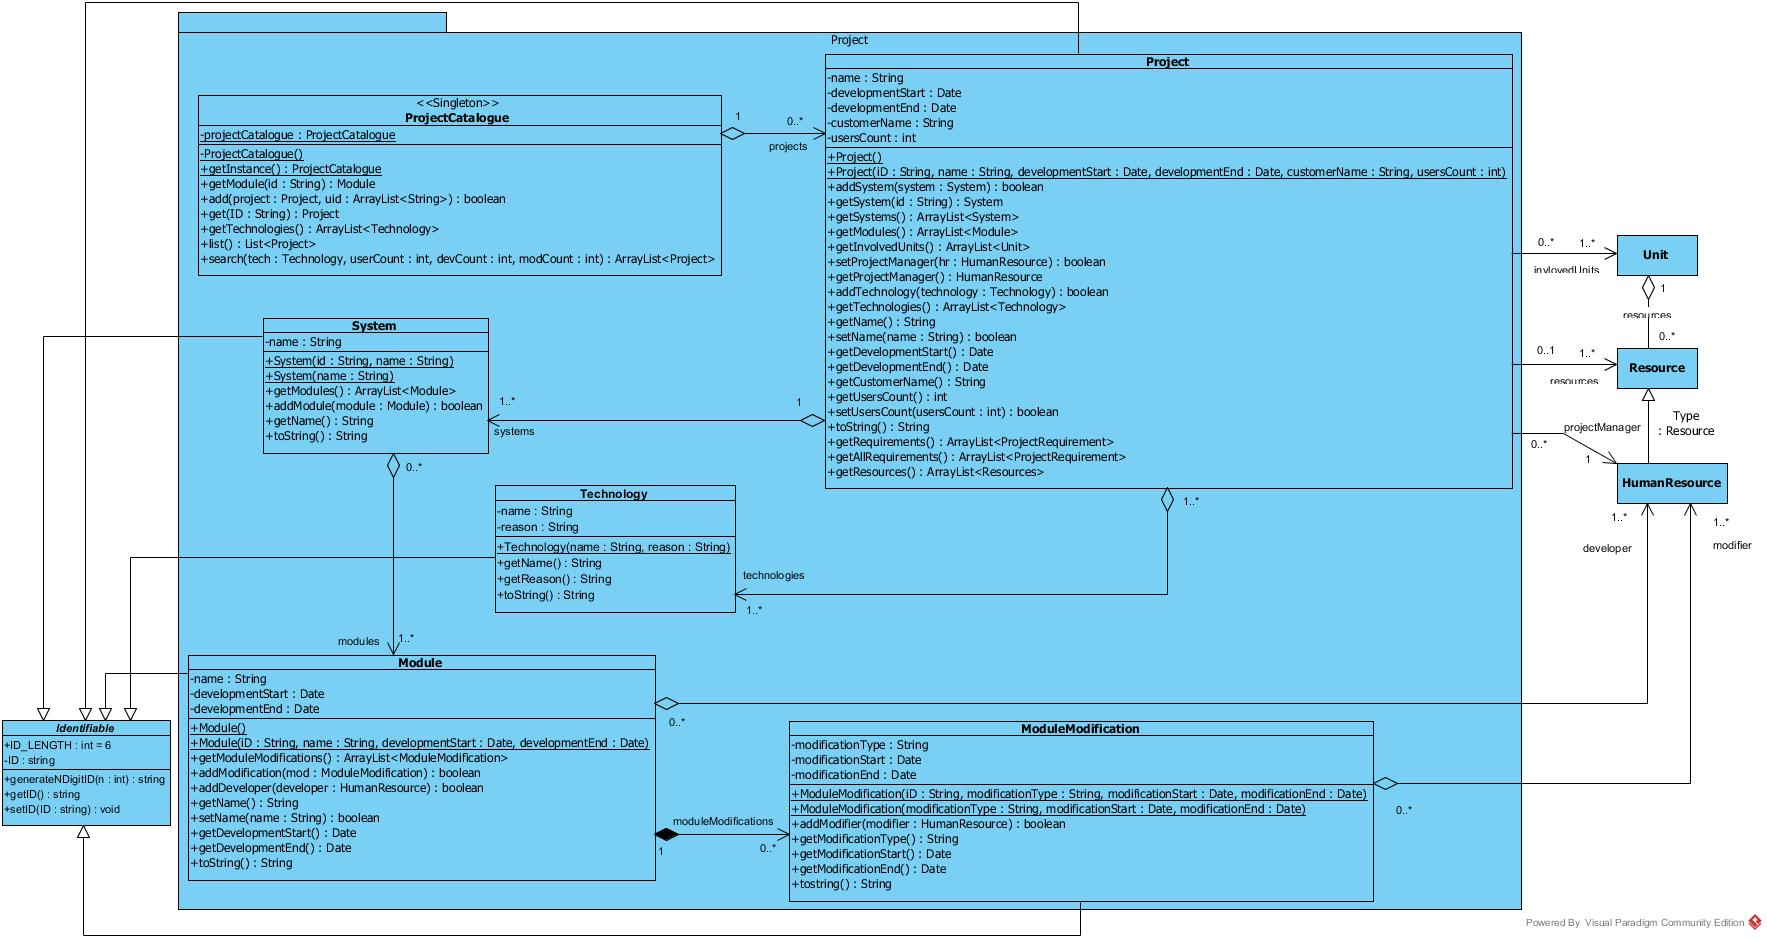
\includegraphics[scale=0.8]{img/class-design/ProjectPackage}
	\caption{بسته واسط کاربری}
\end{figure}
